\documentclass[lualatex,a4paper,openany]{bxjsbook}
\usepackage{amsmath,amssymb,mathrsfs,braket}
% \usepackage{amsthm,amscd} %定理環境, 可換図式
% \usepackage{ascmac} %screen, itembox環境
\usepackage{graphicx,xcolor}
% \usepackage{fancyhdr,lastpage} %ヘッダー/フッター操作
\usepackage{makeidx} %索引
\usepackage{hyperref} %ハイパーリンク
% \hypersetup{colorlinks=true,linkcolor=blue,citecolor=green}
\usepackage{wrapfig}

% 和文フォント
% \usepackage[no-math,ipaex]{luatexja-preset} % IPAexフォント
\usepackage[no-math]{luatexja-fontspec} %Source Han フォント
	\setmainjfont{SourceHanSerifJP}
	\setsansjfont{SourceHanSansJP}
\ltjsetparameter{jacharrange={-2}} % 非ASCII文字がすべて和文と解釈されるのを防ぐ

% 欧文フォント
\setmainfont[Ligatures=TeX]{SourceSerifPro}
% \setmainfont[Ligatures=TeX]{XITS}
% \setmainfont[Ligatures=TeX]{EB Garamond}
\setsansfont[Ligatures=TeX]{SourceSansPro}
% \setmonofont[Ligatures=TeX]{Inconsolatazi4}
\setmonofont[Ligatures=TeX]{SourceCodePro}

% 数式フォント
\usepackage{unicode-math}
\unimathsetup{math-style=ISO,bold-style=ISO}
\setmathfont{LatinModernMath}

% 索引を作成
\makeindex

% jsbook用の設定
\setlength{\textwidth}{\fullwidth} %本文領域を最大化 (余白を小さくする)
\setlength{\evensidemargin}{\oddsidemargin}


% 図表に通し番号を振る
\usepackage{remreset}
\makeatletter
	\@removefromreset{figure}{chapter}
	\def\thefigure{\arabic{figure}}
	\@removefromreset{table}{chapter}
	\def\thetable{\arabic{table}}
	\@removefromreset{equation}{chapter}
	\def\theequation{\arabic{equation}}
\makeatother

% MusiXTeX用設定
\usepackage{musixtex}
\input{musixadd.tex}
\nobarnumbers %小節番号なし
\smallmusicsize %楽譜のサイズを小さく
\newcounter{mycounter} % カウンタの宣言
\setcounter{mycounter}{0} % カウンタの初期化
\newcommand{\useMycounter}[1][]{\refstepcounter{mycounter}{#1}譜例{\themycounter}: }
\newcommand{\musicbegin}{\vspace*{5truemm}\begin{music}}
\newcommand{\musicend}[2]{\end{music}\nopagebreak\begin{center}{\small\useMycounter[\label{#1}]{#2}}\end{center}}

% 小節番号表示用
\newcommand{\shosetu}[1]{
\startbarno=#1
\systemnumbers
\def\writebarno{\llap{\the\barno\barnoadd}}%
\def\raisebarno{2\internote}%
\def\shiftbarno{1.3\Interligne}%
}

% 構造番号
\newcommand{\ind}[2]{$\text{#1}_{\text{#2}}$}

% 文書データ
\title{ブラームス: 交響曲第1番}
\author{H.~S.}
\date{2017.05.07-}

\begin{document}

\maketitle

\tableofcontents


\chapter*{はじめに}
\addcontentsline{toc}{chapter}{はじめに}
\markboth{はじめに}{}



\chapter{作曲に関する経緯}

\section{背景}

\section{作曲過程}

\section{初演}

\section{出版}


\chapter{作品の構造}

\section{概観}

後で詳しく論じるように, この作品は作曲技法の面では4つの楽章間の有機的な動機の結びつきが特徴的である.
しかも, これらの動機はすべて第1楽章の序奏において提示される\footnote{この観点からするとRichard Wagnerの
「ニュルンベルクのマイスタージンガー」と同じ方向を向いているとも言える.}.
各楽章が基本動機に基づいて構築されているという性格のために, 19世紀後半の交響曲としては対位法を愛用するなど, 古典派を思わせる手法が目立っている.
\begin{wrapfigure}{r}{7.0cm}
% \begin{figure}[htbp]
	\centering
	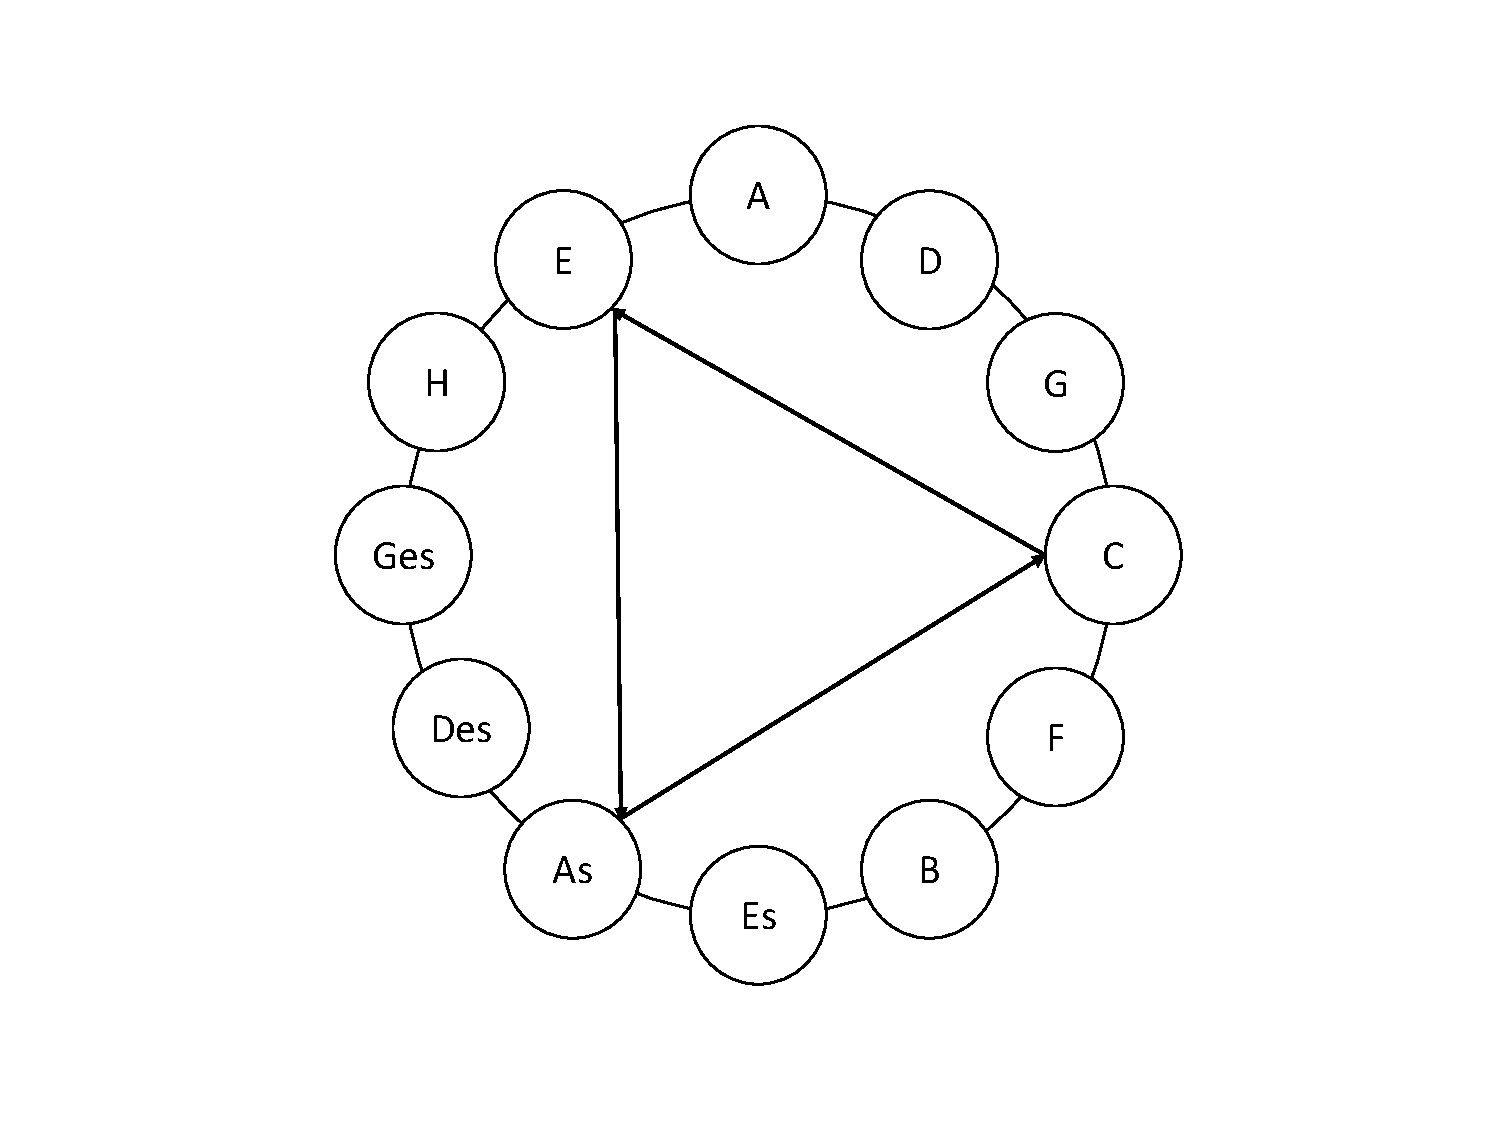
\includegraphics[clip,width=7.0cm]{./figure/modulatory.pdf}
	\caption{第1番の調構造}
	\label{modulatory}
% \end{figure}
\end{wrapfigure}
調性の観点からすると, Brahmsの第1番は彼の多くの作品の中でも独特の立ち位置を占めている:
C-E-As-Cという五度圏上の正三角形を描くような構成 (図\ref{modulatory}) は他にない.
これらの調は互いに遠隔調の関係にあり, いずれも各楽章の最終和音の第3音を起点として自然に移行できる.

第1楽章は大規模な序奏を持つソナタ楽章で, 主部は終始厳格な調子で音楽が展開されるが, コーダで唐突にハ長調に移ると静かに終わる.
これは第2楽章でホ長調へ移るための必然的な要請であるが, 同時に音楽的内容を後続楽章 (特に第4楽章) へ持ち越すための手段ともなっている.
ホ長調の緩徐楽章である第2楽章は, 最終的に三部形式に落ち着いたが, 初演時には現在のものよりも大規模なA-B-A-C-A形式であった.
出版までの演奏を通じてBrahmsはこの楽章をより短く, 圧縮された形へと書き直したのである.
第3楽章は最も短くシンプルな三部形式で, レントラー風のBrahmsらしい間奏曲である.
第4楽章は, やはり大規模な序奏を持つソナタ形式だが, 展開部を欠いており, 再現部が展開部を兼ねる形となっている.
この形式はBrahmsの他の作品にもみられる (弦楽四重奏曲第1番第4楽章など).
また, その序奏にハ短調からハ長調への遷移, アルペンホルンとトロンボーンのコラールという多様な内容が詰め込まれていることも特筆すべきだろう.

曲想, 調性, 構成その他多くの点でこの作品はBeethovenの第5番あるいは第9番と並べて論じられることが多い.
そこでこれら3曲の構成を表\ref{comparison}にまとめておこう.

\begin{table}[htbp]
	\centering
	\begin{tabular}{c|cccc}
		& 第1楽章 & 第2楽章 & 第3楽章 & 第4楽章 \\ \hline
		LvB5 & ソナタ形式 & 変奏曲 & スケルツォ & ソナタ形式 \\
		& c-moll & As-Dur & c-moll & C-Dur \\ \hline
		LvB9 & ソナタ形式 & スケルツォ & 変奏曲 & -- \\
		& d-moll & d-moll & B-Dur & D-Dur \\ \hline
		JB1 & ソナタ形式 & 三部形式 & 三部形式 & ソナタ形式 \\
		& c-moll & E-Dur & As-Dur & C-Dur
	\end{tabular}
	\caption{LvB5, LvB9, JB1の比較}
	\label{comparison}
\end{table}

表\ref{comparison}から明らかなように, これら三曲はいずれも「暗から明へ」という基本的構造は共通であるが,
BrahmsとBeethovenとで中間楽章の調の選び方にはっきりとした相違がある:
Beethovenは中間楽章のどちらか一方は主調である\footnote{Beethovenの場合,
唯一第7番のみA-a-F-Aという調構造であり, (同主調はあるものの) 中間楽章に主調が現れない.}のに対して, Brahmsは (4曲すべての交響曲で) 中間楽章は主調と異なる調性を持つ.
また, Brahmsは中間楽章にBeethoven風のスケルツォを置いていない (第4番のみ第3楽章がスケルツォ風の音楽となっているが, それも2拍子である).

また本作について頻繁に指摘されることとして, 第4楽章第1主題 (譜例\ref{4-62}) がBeethovenの第9番の第4楽章の主要主題 (通称「歓喜の歌」) と類似している.
確かにそうかもしれないが, この指摘にさほど意味はない:
Brahmsのこの主題は全曲の中で必然的にこの形を取ることが決定されており, 他の要因が入り込む余地はない (\ref{sec: mov4}節参照).
加えて, 二つのメロディの類似という現象自体しばしば起こり得る事態であって,
実際この曲についても, 例えばアルペンホルンの主題 (譜例\ref{4-30}) は有名なケンブリッジ大学のグレート・セント・メアリー教会の鐘の音
(日本では「学校のチャイムの音」として知られる) とそっくりである.
他にも, 交響曲第3番第1楽章の第1主題によく似た旋律がRobert Schumannの交響曲第1番第2楽章に現れるなど, この手の事案は枚挙に暇がない.
個々にそのような箇所を指摘して回ったところで, そのような考察から得るものはないだろう.

蛇足であるが, Brahmsの4つの交響曲の調性に関して次の事実に言及されることがある.
これら4曲の調性はC-D-F-Eで, Mozartのジュピター音型に一致する. しかも, Robert Schumannの4つの交響曲B-C-Es-Dを2度平行移動したものでもある.
筆者はこれについて単なる偶然の一致であり意味はないと解釈している:
Brahmsのどの交響曲についても調性はその基本的性格から自然に決定されており, なんらかの意図で選ぶ余地はないように思われる.
特にSchumannの交響曲の番号は単なる出版順であり作曲順は大きく異なっているし, Brahmsもそのことは十分承知していた.


\section{第1楽章: Un poco sostenuto-Allegro}

% 最初に軽く概観

この楽章は大規模な序奏を持つソナタ形式で, 全体の構成を表\ref{structure of mov1}に示す
(便宜上展開部を\ind{D}{1}, \ind{D}{2}, \ind{D}{3}に分けた).
この表では再現部の入りを第343小節としたが, この点については後で詳細に議論する.
\begin{table}[htbp]
	\centering
	\begin{tabular}{c|ccc|ccc|ccc|c}
		序奏I & \multicolumn{3}{c|}{提示部E} & \multicolumn{3}{c|}{展開部D} &
			\multicolumn{3}{c|}{再現部R} & コーダC \\ \hline
		1--37 & \multicolumn{3}{c|}{38--188} & \multicolumn{3}{c|}{189--342} &
			\multicolumn{3}{c|}{343--462} & 463--511 \\
		& \ind{E}{1} & \ind{E}{2} & \ind{E}{c} & \ind{D}{1} & \ind{D}{2} & \ind{D}{3} &
			\ind{R}{1} & \ind{R}{2} & \ind{R}{c} & \\ \cline{2-10}
		& 38- & 130- & 159- & 189- & 225- & 293- & 343- & 403- & 430- & \\
		c & c & Es & es & H--h--c & Ges--c & c--fis & c & C & c & c--C
	\end{tabular}
	\caption{第1楽章の構成}
	\label{structure of mov1}
\end{table}


\clearpage
\musicbegin
	\setmaxinstruments{20}
	\setmaxgroups{8}
	\setmaxslurs{99}
	\def\nbinstruments{14}%   % パート数
	\akkoladen{{1}{5}{7}{9}{10}{14}}
	% \curlybrackets{1245}
	% \sepbarrules % 一旦すべての小節線を切り離す
	% set clefs and names
	\setclef{14}{0}\setname{14}{Fl\hspace{8truemm}}%
	\setclef{13}{0}\setname{13}{Ob\hspace{8truemm}}%
	\setclef{12}{0}\setname{12}{Kl (B)\hspace{10truemm}}%
	\setclef{11}{6}\setname{11}{Fg\hspace{8truemm}}%
	\setclef{10}{6}\setname{10}{Kfg\hspace{8truemm}}%
	\setclef{9}{0}\setname{9}{Hrn (C)\hspace{12truemm}}%
	\setclef{8}{0}\setname{8}{Hrn (Es)\hspace{12truemm}}%
	\setclef{7}{0}\setname{7}{Tr (C)\hspace{10truemm}}%
	\setclef{6}{6}\setname{6}{Pk\hspace{8truemm}}%
	\setclef{5}{0}\setname{5}{Vn1\hspace{7truemm}}%
	\setclef{4}{0}\setname{4}{Vn2\hspace{8truemm}}%
	\setclef{3}{3}\setname{3}{Va\hspace{8truemm}}%
	\setclef{2}{6}\setname{2}{Vc\hspace{8truemm}}%
	\setclef{1}{6}\setname{1}{Kb\hspace{8truemm}}%
	% set chord
	\generalsignature{-3}%    % 調号は正の値のときシャープの数
	\setsign{12}{-1}
	\setsign{9}{0}
	\setsign{8}{0}
	\setsign{7}{0}
	\setsign{6}{0}
	% set metre
	\generalmeter{\meterfrac{6}{8}}%
	\startextract%
		%(1)
		\setclef{2}{0}\zchangeclefs
		\notes
			\ibu{0}{J}{0}\qb{0}{JJ}\tbu{0}\qb{0}{J}\ibu{0}{J}{0}\qb{0}{JJ}\tbu{0}\qb{0}{J}&
			\islurd{2}{c}\itied{1}{c}\qup{c**}\ttie{1}\qu{c*}\sh{c}\itied{1}{c}\cu{c}&
			\pt{c}\zq{c}\isluru{3}{j}\qlp{j**}\pt{g}\zq{g}\qlp{i**}&
			\itieu{5}{j}\qlp{j**}\ttie{5}\ql{j*}\sh{j}\itieu{5}{j}\cl{j}&%Vn2
			&%\isluru{4}{q}\itieu{3}{q}\qlp{q**}\ttie{3}\ql{q*}\sh{q}\itied{3}{q}\cl{q}&
			\ibu{0}{J}{0}\qb{0}{JJ}\tbu{0}\qb{0}{J}\ibu{0}{J}{0}\qb{0}{JJ}\tbu{0}\qb{0}{J}&
			\pt{c}\itied{8}{c}\zq{c}\itieu{9}{j}\qup{j**}\ttie{8}\zq{c}\ttie{9}\cu{j}\ds\ds&%Tp
			\qp\cu{*}\ds\pt{'e}\zq{e}\isluru{19}{g}\qlp{g**}&
			&
			\ibu{0}{C}{0}\qb{0}{CC}\tbu{0}\qb{0}{C}\ibu{0}{C}{0}\qb{0}{CC}\tbu{0}\qb{0}{C}&
			\pt{J}\zq{J}\isluru{21}{c}\qlp{c**}\pt{N}\zq{N}\qlp{b**}&%Fg
			\pt{k}\zq{k}\isluru{22}{r}\qlp{r**}\pt{'h}\zq{h}\qlp{j**}&
			\pt{j}\zq{j}\isluru{23}{q}\qlp{q**}\pt{'g}\zq{g}\qlp{i**}&
			\zcharnote{v}{\hspace*{-8truemm}Un poco sostenuto}\pt{j}\zq{j}\isluru{24}{q}\qlp{q**}\pt{'g}\zq{g}\qlp{i**}
		\enotes
		\bar
		%(2)
		\notes
			\trmu{J}\zhup{J}&
			\ttie{1}\qu{c*}\itied{1}{d}\cu{d}&
			\sh{f}\na{h}\pt{f}\zq{f}\qlp{h**}&
			\ttie{5}\ql{j*}\itieu{5}{k}\cl{k}&%Vn2
			&%\ttie{3}\ql{q*}\itied{3}{r}\cl{r}&
			\trmu{J}\zhup{J}&
			&%Tp
			\pt{'e}\lq{_e}\qlp{^f}&
			&
			\trmu{C}\zhup{C}&
			\sh{M}\na{a}\pt{M}\zq{M}\qlp{a**}&%Fg
			\sh{'g}\na{i}\pt{g}\zq{g}\qlp{i**}&
			\sh{'f}\na{h}\pt{f}\zq{f}\qlp{h**}&
			\sh{'f}\na{h}\pt{f}\zq{f}\qlp{h**}
		\enotes
		\nnotes
			&
			\ibu{0}{d}{+3}\ttie{1}\qbp{0}{d*}\nbbu{0}\qb{0}{e}\qb{0}{f}\tbbu{0}\tbu{0}\tslur{2}{g}\itied{1}{g}\qb{0}{g}&
			\na{f}\fl{h}\zql{f}\ql{h**}\zq{e}\tslur{3}{g}\cl{g}&
			\ibl{5}{k}{+3}\ttie{5}\qbp{5}{k*}\nbbl{5}\qb{5}{l}\qb{5}{m}\tbbl{5}\tbl{5}\itieu{5}{n}\qb{5}{n}&%Vn2
			&%\ibl{0}{r}{+3}\ttie{3}\qbp{0}{r*}\nbbl{0}\qb{0}{s}\qb{0}{t}\tbbl{0}\tbl{0}\tslur{4}{u}\itied{3}{u}\qb{0}{u}
			&
			&%Tp
			\na{'f}\zq{d}\ql{f**}\zq{c}\cl{e}&
			&
			&
			\na{M}\fl{a}\zql{M}\ql{a**}\zq{L}\tslur{21}{N}\cl{N}&%Fg
			\na{'g}\fl{i}\zql{g}\ql{i**}\zq{f}\tslur{22}{h}\cl{h}&
			\na{'f}\fl{h}\zql{f}\ql{h**}\zq{e}\tslur{23}{g}\cl{g}&
			\na{'f}\fl{h}\zql{f}\ql{h**}\zq{e}\tslur{24}{g}\cl{g}
		\enotes
		\def\atnextbar{\znotes&&&&&&\centerbar{\cpause}\en}%
		\bar
		%(3)
		\notes
			\trmu{J}\zhup{J}&
			\ttie{1}\islurd{2}{g}\qu{g*}\itied{1}{h}\cu{h}\ttie{1}\qu{h*}\na{h}\itied{1}{h}\cu{h}&
			\pt{d}\zq{d}\isluru{3}{f}\qlp{f**}\pt{c}\zq{c}\qlp{e**}&
			\ttie{5}\ql{n*}\itieu{5}{o}\cl{o}\ttie{5}\ql{o*}\na{o}\itieu{5}{o}\cl{o}&%Vn2
			&%\ttie{3}\isluru{4}{u}\ql{u*}\itieu{3}{v}\cl{v}\ttie{3}\ql{v*}\na{v}\itieu{3}{v}\ql{v}&
			\trmu{J}\zhup{J}&
			&%Tp
			\pt{i}\zq{i}\qlp{k**}\pt{c}\zq{c}\qup{j**}&
			&
			\trmu{C}\zhup{C}&
			\pt{K}\zq{K}\isluru{21}{M}\qlp{M**}\pt{J}\zq{J}\tslur{21}{L}\qlp{L**}&%Fg
			\pt{'e}\zq{e}\isluru{22}{g}\qlp{g**}\pt{d}\zq{d}\tslur{22}{f}\qlp{f**}&
			\pt{'d}\zq{d}\isluru{23}{f}\qlp{f**}\pt{c}\zq{c}\tslur{23}{e}\qlp{e**}&
			\pt{'d}\zq{d}\isluru{24}{f}\qlp{f**}\pt{'c}\zq{c}\tslur{24}{e}\qlp{e**}
		\enotes
		\def\atnextbar{\znotes&&&&&&\centerbar{\cpause}\en}%
		\bar
		%(4)
		\notes
			\trmu{J}\zhup{J}&
			\ttie{1}\qu{h*}\itied{1}{i}\cu{i}\ttie{1}\qu{i*}\fl{h}\tslur{2}{h}\itied{1}{h}\qu{h}&
			\pt{b}\zq{b}\qlp{d**}\ibl{3}{c}{+2}\zqb{3}{b}\qb{3}{d}\zqb{3}{c}\qb{3}{e}\tbl{3}\zqb{3}{d}\tslur{3}{f}\qb{3}{f}&
			\ttie{5}\ql{o*}\itieu{5}{p}\cl{p}\ttie{5}\ql{p*}\fl{o}\itieu{5}{o}\cl{o}&%Vn2
			&%\ttie{3}\ql{v*}\itieu{3}{w}\cl{w}\ttie{3}\ql{w*}\fl{v}\tslur{4}{v}\itied{3}{v}\ql{v}&
			\trmu{J}\zhup{J}&
			&%Tp
			\zq{g}\curve 234\tslur{19}{i}\qu{i*}\ds\qp\cu{*}\ds&
			&
			\trmu{C}\zhup{C}&
			\pt{I}\zq{I}\isluru{21}{K}\qlp{K**}\ibl{3}{J}{+2}\zqb{3}{I}\qb{3}{K}\zqb{3}{J}\qb{3}{L}\tbl{3}\zqb{3}{K}\tslur{21}{M}\qb{3}{M}&%Fg
			\pt{j}\zq{j}\isluru{22}{l}\qlp{l**}\ibu{3}{e}{+2}\zqb{3}{c}\qb{3}{e}\zqb{3}{d}\qb{3}{f}\tbu{3}\zqb{3}{e}\tbsluru{22}{l}\qb{3}{g}&
			\pt{'b}\zq{b}\isluru{23}{d}\qlp{d**}\ibl{3}{c}{+2}\zqb{3}{b}\qb{3}{d}\zqb{3}{c}\qb{3}{e}\tbl{3}\zqb{3}{d}\tslur{23}{f}\qb{3}{f}&
			\pt{''b}\zq{b}\isluru{24}{d}\qlp{d**}\ibl{3}{b}{+2}\zqb{3}{b}\qb{3}{d}\zqb{3}{c}\qb{3}{e}\tbl{3}\zqb{3}{d}\tslur{24}{f}\qb{3}{f}
		\enotes
		\def\atnextbar{\znotes&&&&&&\centerbar{\cpause}\en}%
		\bar
		%(5)
		\nnotes
			\trmu{J}\zhup{J}&
			\ibu{0}{g}{0}\ttie{1}\ibsluru{2}{h}\qbp{0}{h*}\nbbu{0}\qb{0}{g}\qb{0}{N}\tbbu{0}\tbu{0}\qb{0}{d}&
			\na{b}\pt{b}\zq{b}\isluru{3}{d}\qlp{d**}&
			\ibl{5}{h}{0}\ttie{5}\qbp{5}{o*}\nbbl{5}\qb{5}{n}\qb{5}{g}\tbbl{5}\tbl{5}\qb{5}{k}&%Vn2
			&
			\trmu{J}\zhup{J}&
			&%Tp
			&
			&
			\trmu{C}\zhup{C}&
			\na{I}\pt{I}\zq{I}\isluru{21}{K}\qlp{K**}&%Fg
			\sh{c}\pt{c}\zq{c}\isluru{22}{e}\qlp{e**}&
			\na{'b}\pt{b}\zq{b}\isluru{23}{d}\qlp{d**}&
			\na{''b}\pt{b}\zq{b}\isluru{24}{d}\qlp{d**}
		\enotes
		\notes
			&
			\qu{g*}\tbsluru{2}{f}\cu{f}&
			\ibl{3}{c}{+2}\zqb{3}{b}\qb{3}{d}\zqb{3}{c}\qb{3}{e}\tbl{3}\zqb{3}{d}\tslur{3}{f}\qb{3}{f}&
			\ql{n*}\cl{m}&%Vn2
			&
			&
			&%Tp
			&
			&
			&
			\ibl{3}{J}{+2}\zqb{3}{I}\qb{3}{K}\zqb{3}{J}\qb{3}{L}\tbl{3}\zqb{3}{K}\tslur{21}{M}\qb{3}{M}&%Fg
			\ibl{3}{d}{+2}\zqb{3}{c}\qb{3}{e}\zqb{3}{d}\qb{3}{f}\tbl{3}\zqb{3}{e}\tslur{22}{g}\qb{3}{g}&
			\ibl{3}{'c}{+2}\zqb{3}{b}\qb{3}{d}\zqb{3}{c}\qb{3}{e}\tbl{3}\zqb{3}{d}\tslur{23}{f}\qb{3}{f}&
			\ibl{3}{''c}{+2}\zqb{3}{b}\qb{3}{d}\zqb{3}{c}\qb{3}{e}\tbl{3}\zqb{3}{d}\tslur{24}{f}\qb{3}{f}
		\enotes
		\def\atnextbar{\znotes&&&&&&\centerbar{\cpause}&\centerbar{\cpause}\en}%
	\endextract % 頭にzをつけると最後に小節線を表示しない
\musicend{1-1}{第1楽章冒頭}
\newpage


序奏はティンパニ, コントラバス, コントラファゴットのC音連打の上に何重にも積み重なった上昇音型と下降音型によって開始される.
これらの要素はいずれもこの作品全体を支配する基本的なもので, 本稿ではこれを順に基本動機Z, X, Yと呼称することにする.

\musicbegin
	\shosetu{42}
	\def\nbinstruments{1}%   % パート数 2
	\setstaffs{1}{2}%        % 下から1番目は2段
	\setclef{1}{6000}%       % 下から1番目はへ音記号
	\generalsignature{-3}%    % 調号は正の値のときシャープの数
	\generalmeter{\meterfrac{6}{8}}%  % 拍子は8分の6拍子
	\startextract%
		%(1)
		\notes\lpz{C}\cu{C}\ds\ds|\ds\ds\ibsluru{1}{e}\cu{e}\enotes
		\Notes\isluru{0}{c}\qlp{c}|\qu{g}\enotes
		\notes|\tsslur{1}{g}\cl{l}\enotes
		\bar
		%(2)
		\NOTes\tslur{0}{c}\qlp{c}|\isluru{1}{n}\qlp{n}\enotes
		\Notes\sh{c}\qlp{c}|\tslur{1}{n}\ql{n}\enotes
		\Notes|\na{l}\isluru{1}{l}\cl{l}\enotes
		\bar
		%(3)
		\Notes\itieu{0}{d}\qlp{d}|\tslur{1}{n}\ql{n}\ds\enotes
		\Notes\ibl{0}{d}{-3}\ttie{0}\qbp{0}{d}|\isluru{1}{o}\usf{o}\qlp{o}\enotes
		\notes\nbbl{0}\na{c}\isluru{0}{c}\qb{0}{c}\na{b}\qb{0}{b}\tbl{0}\na{a}\qb{0}{a}|\enotes
		\bar
		%(4)
		\notes\na{b}\tslur{0}{b}\upz{b}\cl{b}\ds|\tslur{1}{o}\ql{o}\enotes
		\notes\ds|\upz{m}\cl{m}\enotes
		\Notes\qp|\upz{k}\ql{k}\enotes
		\notes\lpz{J}\cu{J}|\upz{j}\cl{j}\enotes
		\bar
		%(5)
		\notes\lpz{G}\cu{G}\ds|\na{i}\upz{i}\cl{i}\ds\enotes
	\zendextract % 頭にzをつけると最後に小節線を表示しない
\musicend{1-42}{第1楽章第42小節から}

% 最後に序奏とコーダのテンポ設定の問題に触れる


\section{第2楽章}


\section{第3楽章: Un poco Allegretto e grazioso}

ブラームスはこの大規模な交響曲の中で, 164小節という小振りな「間奏曲」を用意した.
ベートーヴェン風のスケルツォではなく, より古風なメヌエットのような音楽をここに置いたことは,
ベートーヴェンの交響曲 (例えば第5番) から意識的に距離を置いていることの現れであろう.
しかも, この楽章は全体を通して二拍子で書かれており, 純然たるメヌエットでさえない.
この楽章は完全にブラームス風の音楽であり, この事実ひとつ取ってもブラームスの第1番が「ベートーヴェンの第10番」という評価では言い尽くせないことがよく表れている.

\begin{table}[htbp]
	\centering
	\begin{tabular}{cccc}
		主部 (A) & 中間部 (B) & 再現部 (A') & コーダ \\ \hline
		1--70 & 71--114 & 115--153 & 154--164 \\
		As-Dur, 2/4 & H-Dur, 6/8 & As-Dur, 2/4 & As-Dur, 2/4 (6/8)
	\end{tabular}
	\caption{第3楽章の構成}
	\label{structure of mov3}
\end{table}
構成は表\ref{structure of mov3}に示すように比較的単純な三部形式 (A-B-A') だが, 後で見るように再現部A'は主部Aの単調な繰り返しとなることが避けられており,
三部形式の短い楽章にしては変化に富んだ印象を与える.

\musicbegin
	\def\nbinstruments{1}%   % パート数 2
	\setstaffs{1}{2}%        % 下から1番目は2段
	\setclef{1}{6000}%       % 下から1番目はへ音記号
	\generalsignature{-4}%    % 調号は正の値のときシャープの数
	\generalmeter{\meterfrac{2}{4}}%  % 拍子は8分の6拍子
	\startextract%
		%(1)
		\Notes\cmidstaff{\p}\zqu{c}\ibl{0}{H}{0}\qb{0}{HG}|
			\zcharnote{y}{\hspace*{-8truemm}Un poco Allegretto e grazioso}
			\itied{0}{h}\zhl{h}\ibsluru{1}{l}\qu{l}\enotes
		\Notes\zqu{d}\qb{0}{F}\tbl{0}\qb{0}{H}|
			\ibu{1}{k}{-2}\qb{1}{k}\tbsluru{1}{j}\tbu{1}\qb{1}{j}\enotes
		\bar
		%(2)
		\NOtes\ibu{0}{H}{0}\qb{0}{EH}\qb{0}{D}\tbu{0}\qb{0}{H}|
			\zql{e}\ttie{0}\itied{1}{h}\zhl{h}\ibsluru{2}{k}\ibu{1}{k}{-1}\qb{1}{kj}\zql{f}\qb{1}{i}\tbu{1}\tbsluru{2}{j}\qb{1}{j}\enotes
		\bar
		%(3)
		\NOtes\ibu{0}{H}{0}\qb{0}{EH}\qb{0}{D}\tbu{0}\qb{0}{H}|
			\zql{e}\ttie{1}\itied{0}{h}\zhl{h}\ibsluru{2}{k}\ibu{1}{k}{-1}\qb{1}{kj}\zql{f}\qb{1}{i}\tbu{1}\tbsluru{2}{j}\qb{1}{j}\enotes
		\bar
		%(4)
		\Notes\ibu{0}{F}{+1}\qb{0}{C}\tbl{0}\qb{0}{H}|
			\ttie{0}\lq{h}\zhl{e}\ibsluru{1}{i}\ibu{1}{i}{-2}\qb{1}{i}\tbu{1}\tbsluru{1}{h}\qb{1}{h}\enotes
		\Notes\qb{0}{E}\tbu{0}\qb{0}{G}|
			\ibslurd{3}{g}\itied{2}{g}\zql{g}\itieu{0}{i}\qu{i}\enotes
		\bar
		%(5)
		\Notes\ibl{0}{I}{+1}\qb{0}{I}|
			\ttie{0}\zhu{i}\ibl{1}{g}{0}\ttie{2}\qb{1}{g}\enotes
		\Notes\tbl{0}\na{K}\qb{0}{K}|
			\qb{1}{f}\enotes
		\Notes\qb{0}{L}|
			\qb{1}{e}\enotes
		\Notes\tbl{0}\fl{K}\qb{0}{K}|
			\tbslurd{3}{g}\tbl{1}\qb{1}{g}\enotes
	\endextract % 頭にzをつけると最後に小節線を表示しない
\musicend{3-1}{第3楽章冒頭}

第3楽章冒頭はまずチェロのピッチカートに乗ってクラリネットが優雅な旋律を提示する (譜例\ref{3-1}).
ブラームスらしく$5$小節を単位とする変則的な構造を取る. しかも, $2$拍子が$5$小節続くのではなく, $2 + 2 + 3 + 3$という変拍子である.
第6小節からはその反行形が続く.
フルートとファゴットが加わる第11小節からは下降音型を中心とする第2句である (譜例\ref{3-11}).
こちらは冒頭のクラリネット (第1句) と異なり4+4小節の標準的な形である. 第1句と第2句がこの楽章の基本主題を構成する.

\musicbegin
	\startbarno=11
	\systemnumbers
	\def\writebarno{\llap{\the\barno\barnoadd}}%
	\def\raisebarno{2\internote}%
	\def\shiftbarno{1.3\Interligne}%
	\def\nbinstruments{1}%   % パート数
	\setstaffs{1}{1}%        % 下から1番目は2段
	\setclef{1}{0000}%       % 下から1番目はへ音記号
	\generalsignature{-4}%    % 調号は正の値のときシャープの数
	% \generalmeter{\meterfrac{2}{4}}%  % 拍子
	\startextract%
	\NOtes\ibl{0}{l}{-2}\zqp{l}\isluru{1}{n}\qb{0}{n}\enotes
	\notes\tbbl{0}\na{k}\zq{k}\qb{0}{m}\enotes
	\NOtes\zqp{j}\qbp{0}{l}\enotes
	\notes\tbbl{0}\tbl{0}\zq{i}\qb{0}{k}\enotes
	\bar
	\NOtes\ibu{0}{h}{-2}\zqp{h}\qb{0}{j}\enotes
	\notes\tbbu{0}\zq{g}\qb{0}{i}\enotes
	\NOtes\zqp{f}\qbp{0}{h}\enotes
	\notes\tbbu{0}\tbu{0}\zq{e}\tbsluru{1}{l}\qb{0}{g}\enotes
	\bar
	\NOtes\ibl{0}{k}{-2}\na{k}\zqp{k}\isluru{1}{m}\qb{0}{m}\enotes
	\notes\tbbl{0}\zq{j}\qb{0}{l}\enotes
	\NOtes\zqp{i}\qbp{0}{k}\enotes
	\notes\tbbl{0}\tbl{0}\zq{h}\qb{0}{j}\enotes
	\bar
	\NOtes\ibu{0}{h}{-2}\zqp{g}\qb{0}{i}\enotes
	\notes\tbbu{0}\zq{f}\qb{0}{h}\enotes
	\NOtes\qbp{0}{g}\enotes
	\notes\tbbu{0}\tbu{0}\tbsluru{1}{k}\qb{0}{f}\enotes
	\bar
	\NOtes\zhl{g}\ibu{0}{l}{-1}\ibsluru{1}{l}\qb{0}{l}\enotes
	\notes\tbbu{0}\qb{0}{i}\enotes
	\NOtes\qbp{0}{g}\enotes
	\notes\tbbu{0}\tbu{0}\tbsluru{1}{j}\qb{0}{j}\enotes
	\bar
	\NOtes\ibsluru{3}{i}\itieu{2}{i}\lqu{i}\ibl{0}{h}{-1}\ibslurd{1}{h}\qb{0}{h}\enotes
	\notes\tbbl{0}\qb{0}{f}\enotes
	\NOtes\na{d}\zqbp{0}{d}\ibu{1}{i}{+1}\ttie{2}\qbp{1}{i}\enotes
	\notes\tbbl{0}\tbl{0}\tbslurd{1}{h}\zqb{0}{h}\tbbu{1}\tbu{1}\tbsluru{3}{j}\qb{1}{j}\enotes
	\endextract
\musicend{3-11}{第3楽章第11小節から}

第19小節から, やや拡大された形で両旋律が確保される. ここで依然として第1句は9小節単位という変則的な形を,
第2句は4小節単位の標準的な形を保っていることは注目に値する.
また, 拡大部分である第29小節から第31小節にかけて, Vn2にこの曲の基本動機xがさりげなく登場している (譜例\ref{3-29}) ことにも注意したい.

\musicbegin
	\startbarno=29
	\systemnumbers
	\def\writebarno{\llap{\the\barno\barnoadd}}%
	\def\raisebarno{2\internote}%
	\def\shiftbarno{1.3\Interligne}%
	\def\nbinstruments{1}%   % パート数
	\setstaffs{1}{1}%        % 下から1番目は2段
	\setclef{1}{0000}%       % 下から1番目はへ音記号
	\generalsignature{-4}%    % 調号は正の値のときシャープの数
	% \generalmeter{\meterfrac{2}{4}}%  % 拍子
	\startextract%
	\NOtes\isluru{1}{i}\itieu{2}{i}\ql{i}\enotes
	\bar
	\NOtes\ttie{2}\ql{i}\na{i}\ql{i}\enotes
	\bar
	\NOtes\ql{j}\ql{k}\enotes
	\bar
	\Notes\ibl{0}{l}{-2}\na{k}\qb{0}{k}\curve 543\tslur{1}{j}\qb{0}{j}\isluru{1}{k}\upz{i}\qb{0}{i}\tbl{0}\tslur{1}{j}\upz{h}\qb{0}{h}\enotes
	\endextract
\musicend{3-29}{第3楽章第29小節2拍目からのVn2}

第45小節でヘ短調に落ち込むと, クラリネット, 次いでフルートとオーボエに新しいリズムが出る (譜例\ref{3-45}) が,
これは前半は第2句, 後半は第1句に基づく経過句である.

\musicbegin
	\startbarno=45
	\systemnumbers
	\def\writebarno{\llap{\the\barno\barnoadd}}%
	\def\raisebarno{2\internote}%
	\def\shiftbarno{1.3\Interligne}%
	\def\nbinstruments{1}%   % パート数
	\setstaffs{1}{1}%        % 下から1番目は2段
	\setclef{1}{0000}%       % 下から1番目はへ音記号
	\generalsignature{-4}%    % 調号は正の値のときシャープの数
	% \generalmeter{\meterfrac{2}{4}}%  % 拍子
	\startextract%
	% \startpiece
		%(1)
		\Notes\ds\isluru{1}{j}\cl{j}\enotes
		\bar
		%(2)
		\Notes\ibu{0}{i}{-2}\na{i}\qb{0}{i}\qb{0}{h}\qb{0}{g}\tbu{0}\curve 522\tbsluru{1}{l}\qb{0}{f}\enotes
		\bar
		%(3)
		\Notes\ibl{0}{i}{+2}\na{i}\isluru{1}{i}\qbp{0}{i}\enotes
		\notes\tbbl{0}\tbl{0}\tslur{1}{k}\qb{0}{k}\enotes
		\notes\ibbl{0}{j}{+2}\isluru{2}{j}\qb{0}{jon}\tbbl{0}\tbl{0}\curve512\tslur{2}{m}\isluru{1}{m}\qb{0}{m}\enotes
		\bar
		%(4)
		\Notes\ibl{0}{l}{-2}\na{l}\qb{0}{l}\qb{0}{k}\qb{0}{j}\tbl{0}\tbsluru{1}{i}\fl{i}\qb{0}{i}\enotes
		\bar
		%(5)
		\NOtes\ibl{0}{l}{+2}\fl{l}\isluru{1}{l}\qbp{0}{l}\enotes
		\notes\tbbl{0}\tbl{0}\tslur{1}{n}\fl{n}\qb{0}{n}\enotes
		\notes\ibbl{0}{j}{+2}\isluru{2}{m}\qb{0}{mrq}\tbbl{0}\tbl{0}\curve511\tslur{2}{p}\qb{0}{p}\enotes
		\bar
		% \alaligne
		%(6)
		\Notes\zq{m}\ql{o}\enotes
		\Notes\ibl{0}{l}{-2}\na{l}\zq{l}\isluru{1}{n}\qb{0}{n}\tbl{0}\na{k}\zq{k}\tslur{1}{m}\qb{0}{m}\enotes
		\bar
		%(7)
		\notes\ibbl{0}{l}{0}\na{l}\zq{l}\isluru{1}{n}\qb{0}{n}\na{k}\zq{k}\qb{0}{m}\zq{j}\qb{0}{l}\tbl{0}\zq{k}\tslur{1}{m}\qb{0}{m}\enotes
		\notes\ibbl{0}{l}{0}\zq{l}\isluru{1}{n}\qb{0}{n}\zq{k}\qb{0}{m}\zq{j}\qb{0}{l}\tbl{0}\zq{l}\tslur{1}{n}\qb{0}{n}\enotes
		% \bar
		% %(8)
		% \NOtes\zq{m}\ql{o}\enotes
		% \Notes\ibl{0}{l}{-2}\na{l}\zq{l}\isluru{1}{n}\qb{0}{n}\tbl{0}\na{k}\zq{k}\tslur{1}{m}\qb{0}{m}\enotes
		% \bar
		% %(9)
		% \notes\ibbl{0}{l}{0}\na{l}\zq{l}\isluru{1}{n}\qb{0}{n}\na{k}\zq{k}\qb{0}{m}\zq{j}\qb{0}{l}\tbl{0}\zq{k}\tslur{1}{m}\qb{0}{m}\enotes
		% \notes\ibbu{0}{l}{-4}\zcl{l}\ibsluru{1}{n}\qb{0}{n}\qb{0}{l}\enotes
		% \notes\raise-2\Interligne\rlap\ds\na{i}\qb{0}{i}\tbu{0}\tbsluru{1}{k}\qb{0}{j}\enotes
	\endextract
	% \endpiece
\musicend{3-45}{第3楽章第45小節2拍目から}

減七和音を踏み台に第62小節で変イ長調に戻ると第1句を再現するが, これはあっさりと流して遠隔調であるロ長調の中間部へと続く.
ここで第65小節からの木管楽器の動きが第4楽章の第58小節や第295小節を思い出させる, と言うと穿ちすぎだろうか.
その解釈に立ってこの箇所を第3楽章第28小節からの木管および譜例\ref{3-29}に関する上の記述と比較すると,
主部Aにおいて3回演奏されるこの主要主題は, 最初 (第1小節から) は含みのない形で提示されるが,
2回目 (第19小節から) は第1楽章に, 3回目 (第62小節から) は第4楽章に寄せている, ということになる.
中間部Bが第1楽章の追憶に捧げられ, 再現部A'が第4楽章の準備段階となっていることを踏まえると, この見方は如何にもありそうに思える.

\musicbegin
	\shosetu{71}
	\def\nbinstruments{1}%   % パート数
	% \setstaffs{1}{2}%        % 下から1番目は2段
	% \setclef{1}{6000}%       % 下から1番目はへ音記号
	\generalsignature{+5}%    % 調号は正の値のときシャープの数
	\generalmeter{\meterfrac{6}{8}}%  % 拍子
	\startextract%
		\notes\ds\ibu{0}{k}{0}\islurd{1}{k}\qb{0}{k}\tbu{0}\qb{0}{k}\enotes
		\notes\tslur{1}{k}\zqup{k}\raise-3\Interligne\ds\ibl{1}{f}{-2}\isluru{2}{f}\qb{1}{f}\tbl{1}\qb{1}{d}\enotes
		\bar
		\notes\tslur{2}{b}\zql{b}\ds\ibu{0}{k}{0}\islurd{1}{k}\qb{0}{k}\tbu{0}\zqb{0}{k}\raise-3\Interligne\ds\enotes
		\notes\tslur{1}{k}\zqup{k}\raise-3\Interligne\ds\ibl{1}{d}{-2}\isluru{2}{d}\qb{1}{d}\tbl{1}\qb{1}{b}\enotes
		\bar
		\notes\tslur{2}{N}\zqlp{N}\ds\ibl{0}{i}{+1}\zq{i}\isluru{1}{k}\qb{0}{k}\tbl{0}\zq{j}\qb{0}{l}\enotes
		\notes\ibl{0}{k}{-2}\zq{k}\qb0{m}\zq{j}\qb0{l}\tbl0\zq{i}\qb0{k}\enotes
		\bar
		\notes\ibu{0}{h}{0}\zq{h}\qb0{j}\zq{g}\qb0{i}\tbu0\zq{h}\qb0{j}\enotes
		\notes\ibl{0}{i}{+2}\zq{i}\qb0{k}\zq{j}\qb0{l}\tbl0\zq{k}\tslur{1}{m}\qb0{m}\enotes
		\bar
		\Notes\zq{h}\qu{j}\ds\enotes
	\zendextract % 頭にzをつけると最後に小節線を表示しない
\musicend{3-71}{第3楽章第71小節から}

中間部は八分の六拍子でのDis音の連打から始まる (譜例\ref{3-71}). これは直前の第65小節から第70小節にかけて何度も強調されるB音から誘導されたものであるが,
第83小節でホルンとトランペットが強い調子でFis音を連打するに至って, これが第1楽章のオルゲルクンプトの回想であることが明らかになる (第1楽章展開部の金管楽器の用法を思い出そう).
ただ, 第73小節からの順次進行は節回しや3度を好む傾向という点ではむしろ第2楽章の主要主題を思わせる.

続くトリオ風の音楽 (第87小節から) は不安定な和音進行が特徴的である.
それまではロ調まわりで安定していたが, ここで基本動機xがバス声部に潜ることによって多彩な和声が導き出される.

% 和声進行もうちょっと詳しく書く

第107小節でDis音の連打だけが残ると, これをEs音に読み替えることで変イ短調でEs-Des-Ces-Bの順次下降が弦楽器のユニゾンで奏される (譜例\ref{3-108}).
これはもちろん中間部Bを打ち切り主部Aの再現を開始するという合図であるが, 同時に第4楽章冒頭の予告にもなっている (譜例\ref{4-1}).

\musicbegin
	\shosetu{108}
	\def\nbinstruments{1}%   % パート数
	\setstaffs{1}{1}%        % 下から1番目は2段
	\setclef{1}{0000}%       % 下から1番目はへ音記号
	\generalsignature{-4}%    % 調号は正の値のときシャープの数
	\generalmeter{\meterfrac{2}{4}}%  % 拍子
	\startextract%
	\NOtes\isluru{1}{s}\ql{s}\enotes
	\Notes\ibl{0}{p}{-2}\qb{0}{r}\tbl{0}\fl{q}\qb{0}{q}\enotes
	\bar
	\Notes\tslur{1}{p}\cl{p}\ds\enotes
	\NOtes\qp\enotes
	\bar
	\NOtes\qu{e}\qp\enotes
	\bar
	\NOtes\qu{d}\fl{c}\qu{c}\enotes
	\bar
	\Notes\cu{b}\ds\enotes
	\zendextract
\musicend{3-108}{第3楽章第108小節からのVn1}

第115小節からの再現部A'ではまずクラリネットが冒頭主題を再現するが,
フルートとオーボエによる中間部Bに基づく対旋律が付加されているために雰囲気は冒頭とはやや異なる.
次いで主部では旋律\ref{3-1}の反行形が提示された箇所は, ヴァイオリンの目新しいがどこか懐かしい旋律に置き換えられる (譜例\ref{3-118}).
これは暗に第4楽章第1主題 (譜例\ref{4-61})を指し示しているが, 両者の類似は単なる旋律上のものだけではない.
中間部の和声, リズムともに複雑な領域を抜けた後で提示されるこの変ニ長調の控えめな旋律 (molto dolceの指定付き) によって,
聞き手の緊張が和らげられ, 自然にリラックスした状態に落ち着くことになる.
この効果はまさに全曲の中で第4楽章第1主題が果たす役割と同一のものである.

\musicbegin
	\shosetu{118}
	\def\nbinstruments{1}%   % パート数
	\setstaffs{1}{1}%        % 下から1番目は2段
	\setclef{1}{0000}%       % 下から1番目はへ音記号
	\generalsignature{-4}%    % 調号は正の値のときシャープの数
	% \generalmeter{\meterfrac{2}{4}}%  % 拍子
	\startextract%
	\NOtes\isluru{1}{i}\itieu{2}{i}\ql{i}\enotes
	\bar
	\NOtes\ttie{2}\ql{i}\tslur{1}{j}\ql{j}\enotes
	\bar
	\notesp\ibl{0}{k}{0}\isluru{1}{k}\qb{0}{k}\enotes
	\notes\nbbl{0}\qb{0}{l}\tbbl{0}\qb{0}{m}\enotes
	\notesp\qb{0}{l}\tbl{0}\qb{0}{k}\enotes
	\bar
	\notesp\ibl{0}{j}{0}\qb{0}{j}\qb{0}{l}\qb{0}{k}\tbl{0}\qb{0}{j}\enotes
	\bar
	\notesp\ibl{0}{i}{-1}\qb{0}{i}\enotes
	\notes\nbbl{0}\qb{0}{j}\tbbl{0}\qb{0}{k}\enotes
	\notesp\qb{0}{j}\tbl{0}\qb{0}{g}\enotes
	\bar
	\notes\ibu{0}{h}{0}\nbbu{0}\qb0{h}\tbbu{0}\qb0{i}\enotes
	\nnotes\triolet{b}\nbbu{0}\qb0{h}\qb0{g}\tbbu{0}\tbu{0}\qb0{h}\enotes
	\notesp\ibl{0}{j}{-2}\qb0{j}\tbl{0}\curve 542\tslur{1}{i}\qb0{i}\enotes
	% \bar
	% \Notes\qu{g}\enotes
	% \notesp\ibu{0}{f}{-2}\islurd{1}{f}\qb0{f}\tbu{0}\na{d}\tslur{1}{d}\qb{0}{d}\enotes
	% \bar
	% \NOtes\hu{e}\enotes
	\endextract
\musicend{3-118}{第3楽章第118小節2拍目からのVn1}

第126小節からの第2句は後半が大幅に拡大され, 主部にあったヘ短調の経過句を飲み込んで, 第144小節での第1句の再提示へと繋がる.
ヴァイオリンが一瞬だけ基本主題xを思い出す (第148小節) が, しかしその思いを振り切って変ニ短調に傾斜したコーダへ入る.

コーダは第154小節から第164小節というごく短いもので, 中間部Bの追憶となっている.
ここではブラームスが好んで使用した二連符と三連符の交錯がくすんだニュアンスという絶妙な効果を発揮している.
また, 下降音型は短調と, 上昇音型は長調と結び付けられており,
主和音の明確な提示を回避しながらも十分な音楽的効果が発揮される. この手法は後の交響曲第3番, 特に第4楽章第2主題を思わせる.

第3楽章は, 大規模な第1楽章, 第4楽章の間にあって規模が小さすぎ, 音楽的にも内容に乏しいとの批判がある.
% リファレンスが必要
しかしこの批判は妥当ではない.
上で見たように, さりげない形で\footnote{この点でもベートーヴェンの第5番あるいは第9番との相違は際立っている.}第1楽章の内容を再提示し,
フィナーレへの足掛かりを用意するという点にこの楽章の意義がある.
この観点からするとブラームスが書き下したこの音楽は必要な内容を完全に含んでおり, 作品全体を傑作たらしめるのに十分であると言えよう.


\section{第4楽章: Adagio-Più Andante-Allegro non troppo, ma con brio}\label{sec: mov4}



\chapter{演奏と録音}

\section{初演から出版まで}\label{sec: till publication}

\begin{figure}[htbp]
	\begin{center}
    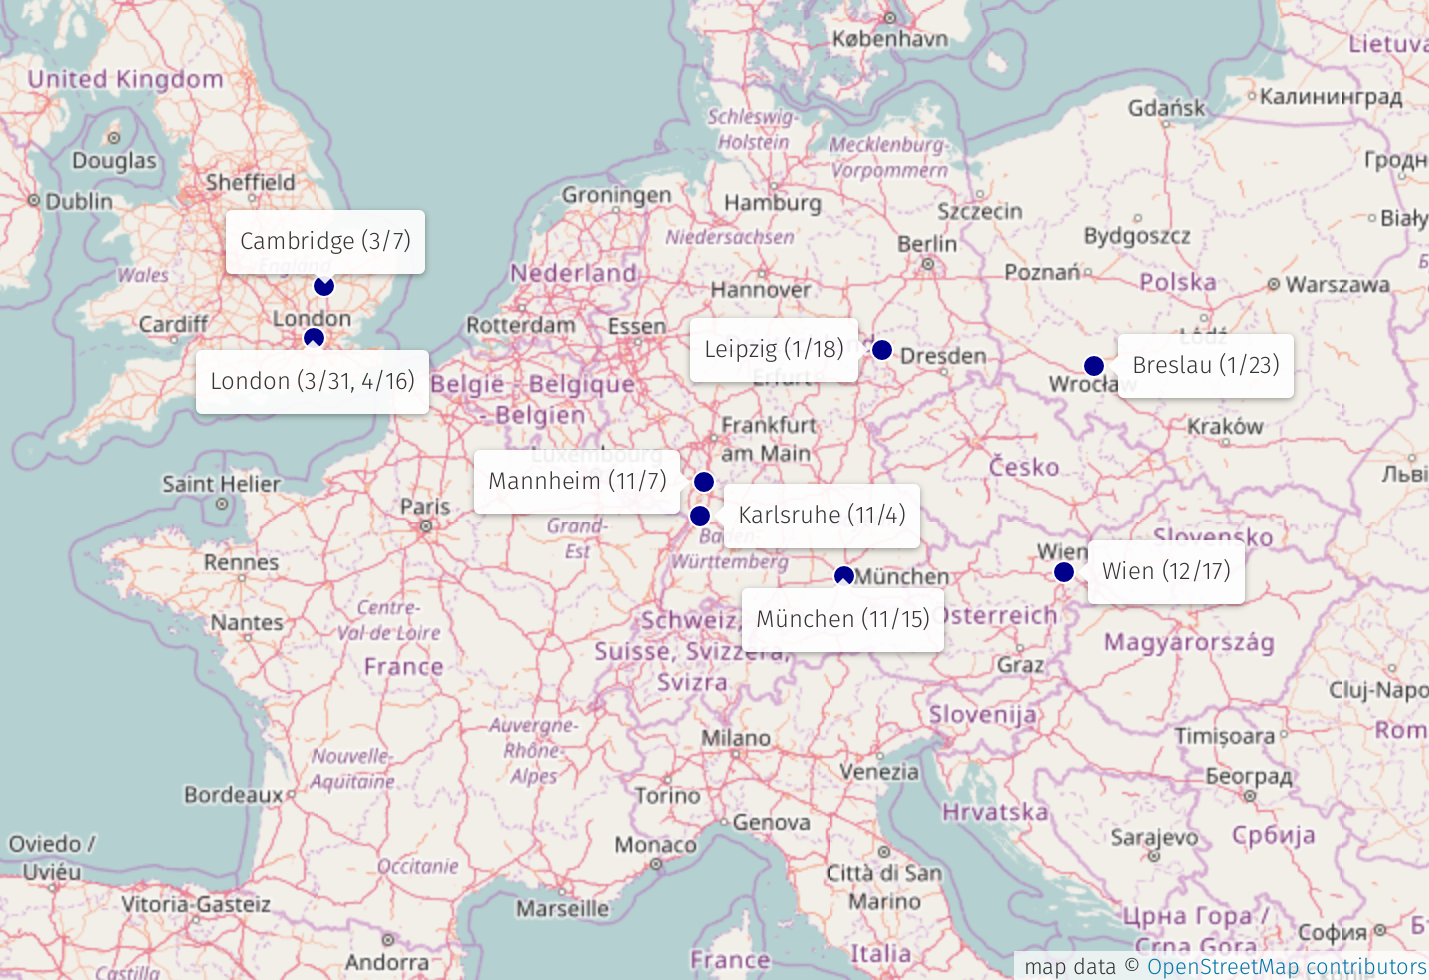
\includegraphics[clip,width=14.0cm]{./figure/map-concert.png}
	\caption{交響曲第1番が手稿譜で演奏された都市.
		地図はOpenStreetMapによる (\href{http://www.openstreetmap.org/copyright}{ライセンス}).}
    \label{fig: concert}
	\end{center}
\end{figure}

\section{19世紀ドイツ・オーストリアにおける受容}

\section{ヨーロッパおよびアメリカ}

\section{日本における演奏史}

\section{録音}

% この傑作の録音の完全なリストを作成することは (演奏のリストほどではないにしても) 到底実現不可能である.
% なんらかの基準を設けて項目を選択したとしても, その基準の妥当性が問題になる.
% 従ってここに掲載するリストは筆者の独断と偏見を多分に含むことになる.



\begin{thebibliography}{99}
	\bibitem{frisch} ウォルター・フリッシュ (訳 : 天崎 浩二) 「ブラームス 4つの交響曲」音楽之友社 (1999)
	\bibitem{denki} 三宅 幸夫 「ブラームス」新潮文庫 (1986)
	\bibitem{onpu} 池辺 晋一朗 「ブラームスの音符たち」音楽之友社 (2005)
	\bibitem{compos} 西原 稔 「作曲家 人と作品シリーズ ブラームス」音楽之友社 (2006)
	\bibitem{library} 「作曲家別名曲解説ライブラリー ブラームス」音楽之友社 (1993)
	\bibitem{kaisouroku} 「ブラームス回想録集」全三巻, 音楽之友社 (2004)
	\bibitem{ogt} スコア 音楽之友社版 (2003) 解説 : 三宅 幸夫
	\bibitem{henle} スコア G.~Henle Verlag版 (1997) 解説 : Robert Pascall
	\bibitem{clara} ベルホルト・リッツマン編 (編訳 : 原田 光子) 「クララ・シューマン ヨハネス・ブラームス 友情の書簡」みすず書房 (2012)
\end{thebibliography}


\printindex

\end{document}
